% !TEX root = main.tex
\documentclass{article}
\usepackage{../include/report_style}

\newcommand{\TODO}[1]{\textcolor{red}{TODO: #1}} % for comments

\title{Lean Applications in the Department of Defense}
\author{Juan Carlos Cruz - ira406}
\date{ME 5703 Lean Product Development and Service Systems}

\begin{document}
	\maketitle
	\noindent%


	\begin{abstract}
		To do.
	\end{abstract}

	% Introduction
	\section{Introduction}

	The Department of Defense (DoD), which includes the U.S. Army, Navy, Air Force, Marine Corps, Space Force, National Security Agency, Defense Intelligence Agency, National Geospatial-Intelligence Agency, and National Reconnaissance Office, is traditionally viewed as a bureaucratic and slow-moving organization due to its sheer size and complexity.

	For my research proposal, I aim to investigate the implementation of lean and six-sigma principles within the DoD and its affiliated organizations to identify if these principles have been successful in improving the efficiency and effectiveness of the DoD.
	To better understand research trends regarding lean and six-sigma implementation regarding the DoD, a scientometric review is conducted.
	Following the procedure outlined in \cite{MA2023104828}, the review begins by selecting an appropriate database, tailoring a search term criteria, filtering the results, and then analyzing the key research themes appearing across the resulting works.

	The complete citation dataset, analysis code, and figures can be found at \url{https://github.com/jc-cr/lean_dod_paper}.

	% Analysis setup

	\section{Scientometric Setup}

	ProQuest was selected as the primary database for this search as it yielded the most results, 481 total, including Theses, Trade journals, Scholarly Articles, and Conference Papers.

	The author also reviewed the Web of Science, Lens, and the Defense Technical Information Center, but found these to have insufficient paper results for this analysis.

	One downside to this search method is that valuable "Grey literature" including government web articles and reports are not included within the analysis, this limitation will be covered in the final report by including such literature in the final review.

	The search term used in ProQuest was as follows:

	\begin{minipage}{\linewidth}
	\begin{spacing}{0.8}
	\noindent\texttt{AB("Department of Defense" OR "DoD" OR "DOD" OR "U.S. Army" OR} \\
	\texttt{"Department of the Army" OR "U.S. Navy" OR "Department of the Navy" OR} \\
	\texttt{"U.S. Air Force" OR "Department of the Air Force" OR "U.S. Marine Corps" OR} \\
	\texttt{"U.S. Space Force" OR "National Security Agency" OR "NSA" OR} \\
	\texttt{"Defense Intelligence Agency" OR "DIA" OR "National Geospatial-Intelligence} \\
	\texttt{Agency" OR "NGA" OR "National Reconnaissance Office" OR "NRO")} \\
	\texttt{AND FT("six sigma" OR "6$\sigma$" OR "lean six sigma" OR} \\
	\texttt{"continuous process improvement" OR "LSS") AND LA(EN)}
	\end{spacing}
	\end{minipage}


	The resulting papers were inspected and cleaned manually for irrelevant documents or duplicates, leaving 465 documents to analyze.
	The results were exported to a xlsx file and then analyzed with a python script.

	The python analysis program was setup to output graphs related to the following items:

	\begin{itemize}
		\item \textbf{Publication Trend Analysis}: Temporal distribution of publications by year, including trend lines and 3-year moving averages to identify patterns in research activity.
		
		\item \textbf{Document Type Classification}: Analysis of publication types (e.g., journal articles, case studies, dissertations).
		
		\item \textbf{Keyword Analysis}: Extraction and frequency analysis of keywords from abstracts, including removal of common stopwords and use of lemmatization for term normalization.
		
		\item \textbf{Network Analysis}: Construction of keyword co-occurrence networks to visualize relationships between concepts in the literature, with filtering to highlight the most significant connections.
		
		\item \textbf{Topic Modeling}: Latent Dirichlet Allocation (LDA) modeling to identify underlying thematic structures across the corpus of abstracts.
		
		\item \textbf{Thematic Trend Analysis}: From prior analysis, analysis of the identified themes in the literature over time.

		\item \textbf{Thematic Distribution}: Distribution of themes across the corpus of abstracts.
	\end{itemize}

	The results and figures generated from these analysis methods are presented in the following sections.

	\section{Scientometric Analysis}

	As seen in \figref{fig:publication_trend}, from the earliest publications found in 1992 up to 2025, there has been an increasing trend for lean six sigma related publication related to the DoD and it's affiliated organizations.
	The year 2017 saw the most amount of publication related to lean six sigma and the DoD.
	Interestingly, since 2017 there has been a downward trend in lean six sigma literature.


	\begin{figure}[htbp]
	\centering
	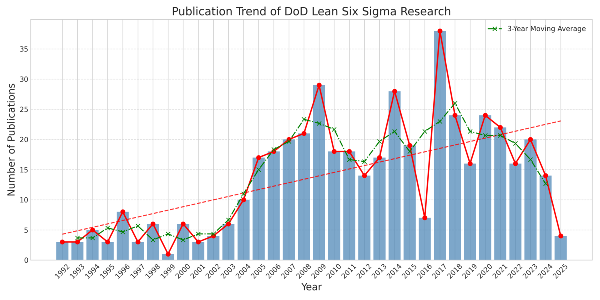
\includegraphics[width=0.9\linewidth,height=0.9\textheight,keepaspectratio]{publication_trend}
	\caption{Publications in lean six sigma from database search}
	\label{fig:publication_trend}
	\end{figure}

	The majority of the publication types found in the ProQuest database are Dissertation/Thesis, with Feature, and General Information documents following after.
	This is visualized in \figref{fig:document_type}
	The trends over time for the different document classes is shown in \figref{fig:document_type_trend}.

	\begin{figure}[htbp]
		\centering
		\begin{subfigure}[b]{0.48\textwidth}
			\centering
			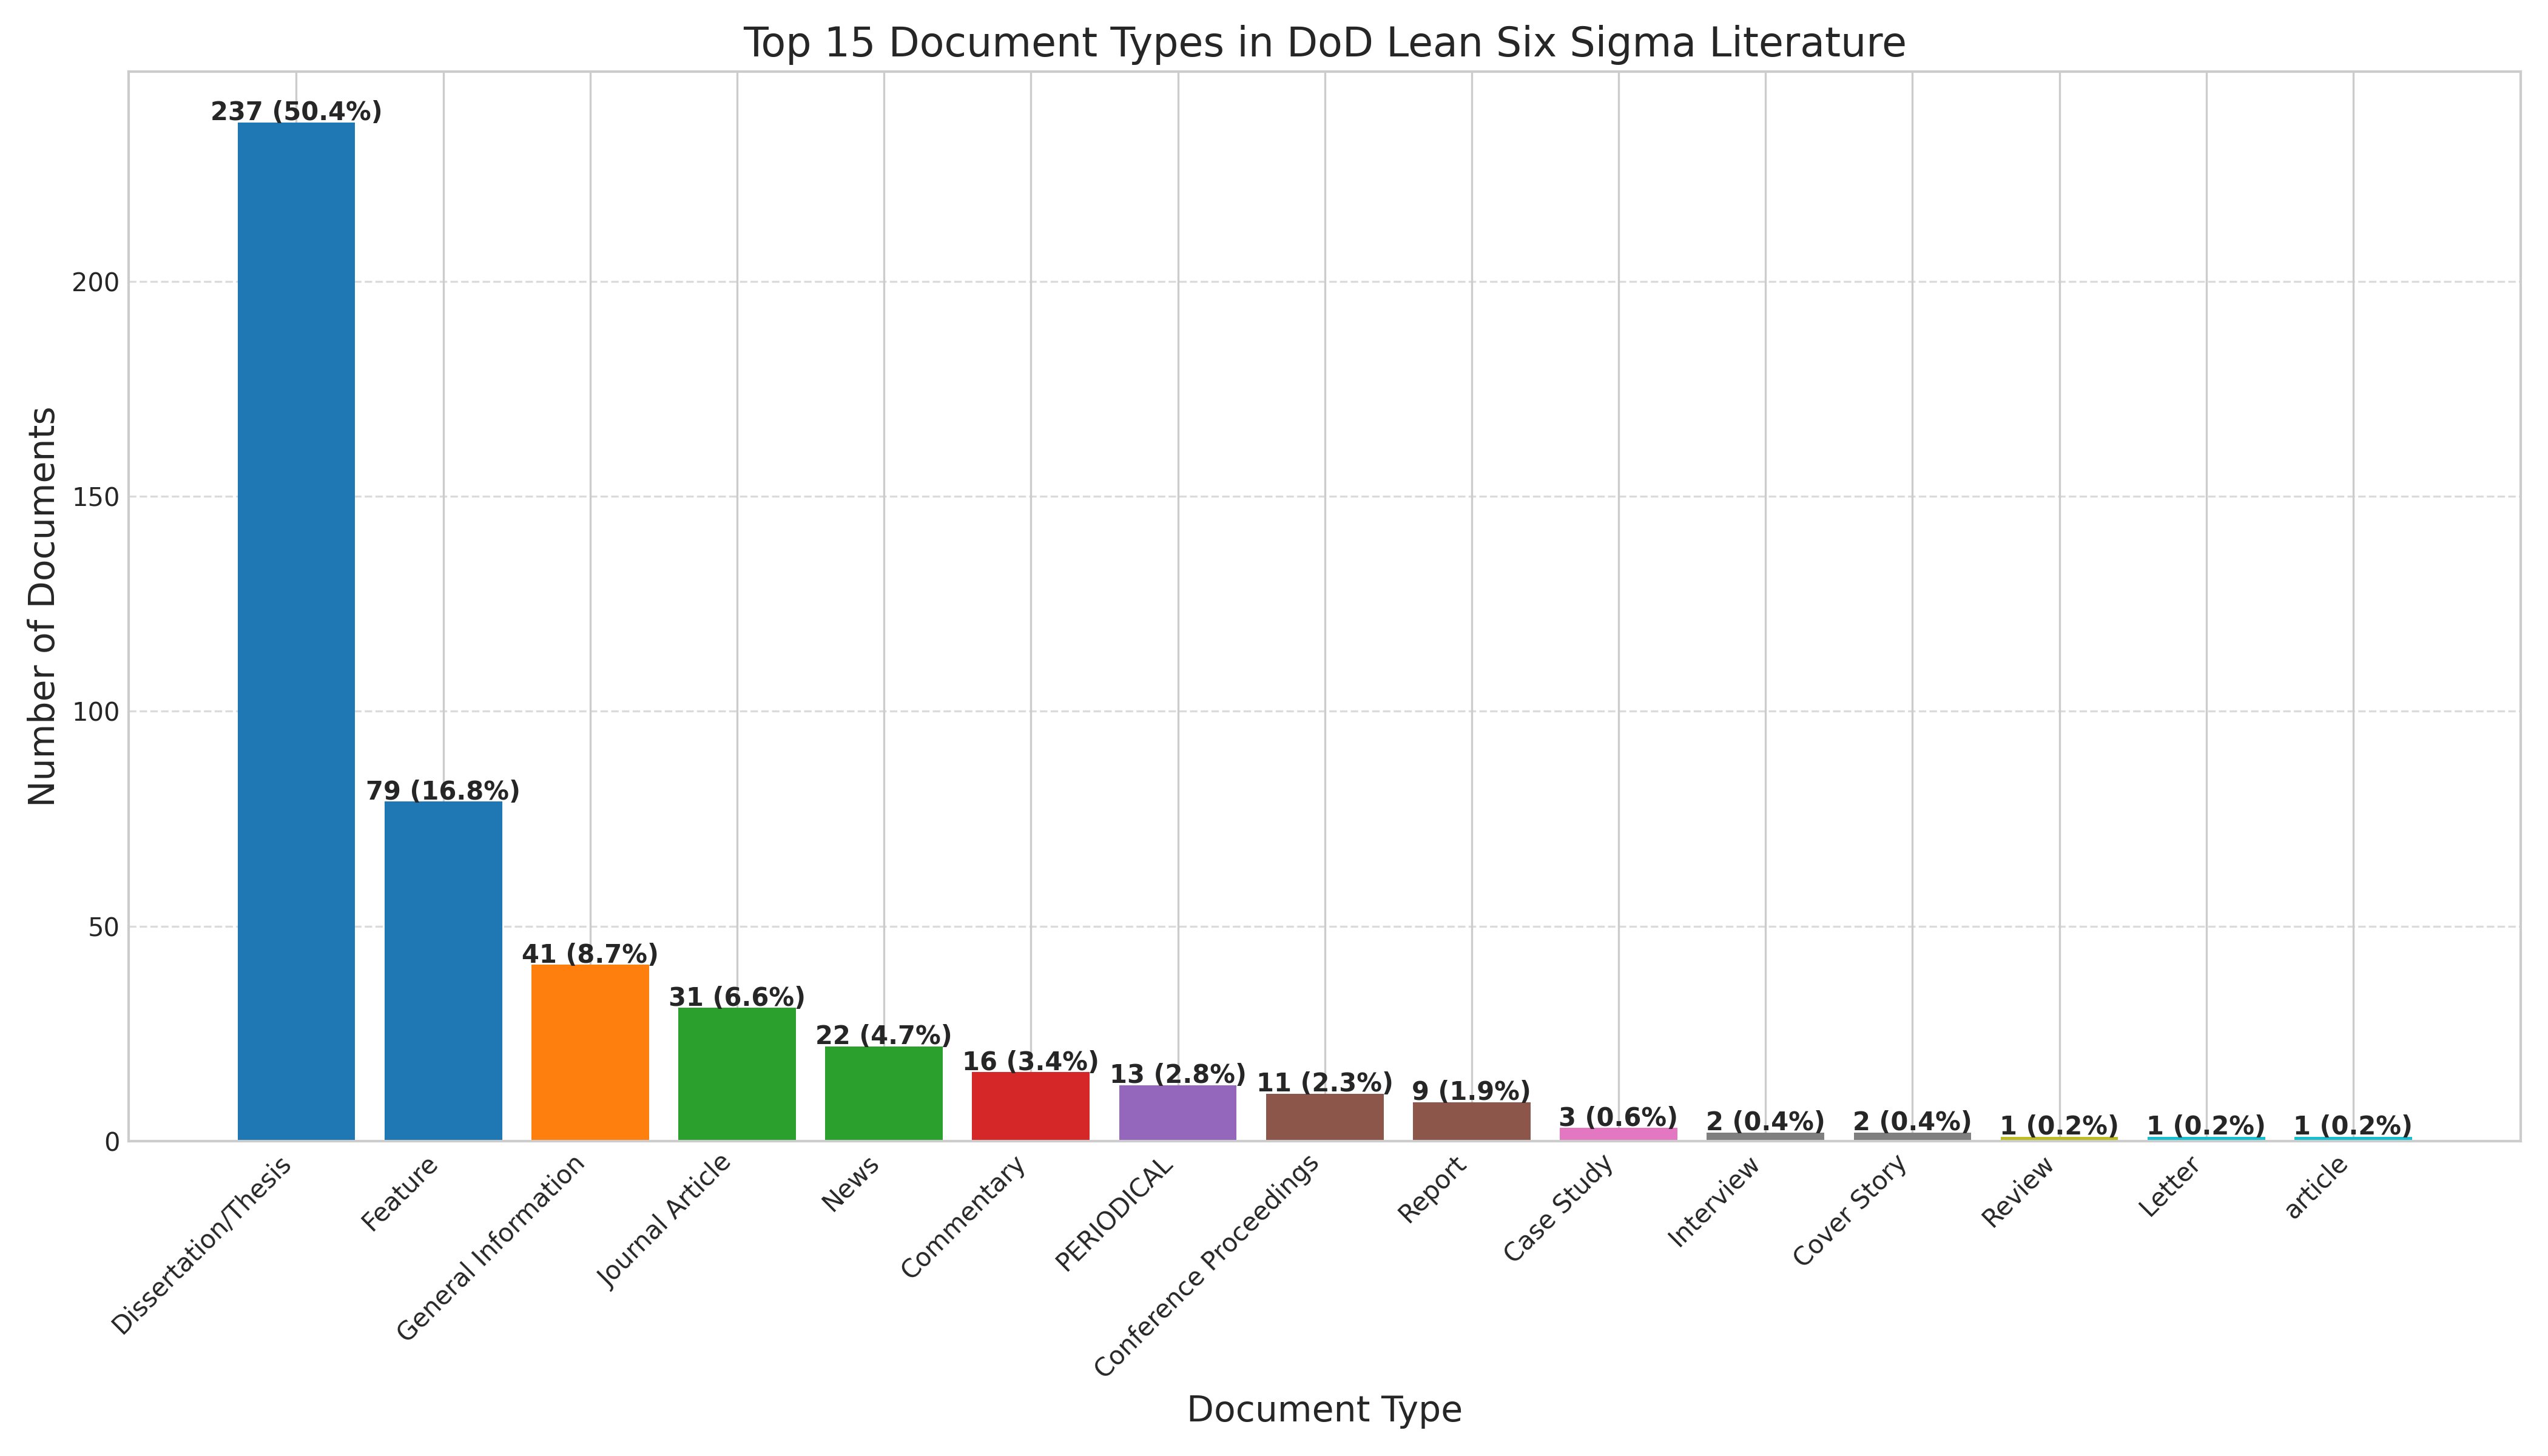
\includegraphics[width=\textwidth,height=0.35\textheight,keepaspectratio]{document_type_distribution_bar}
			\caption{Types of publications found in the database search}
			\label{fig:document_type}
		\end{subfigure}
		\hfill
		\begin{subfigure}[b]{0.48\textwidth}
			\centering
			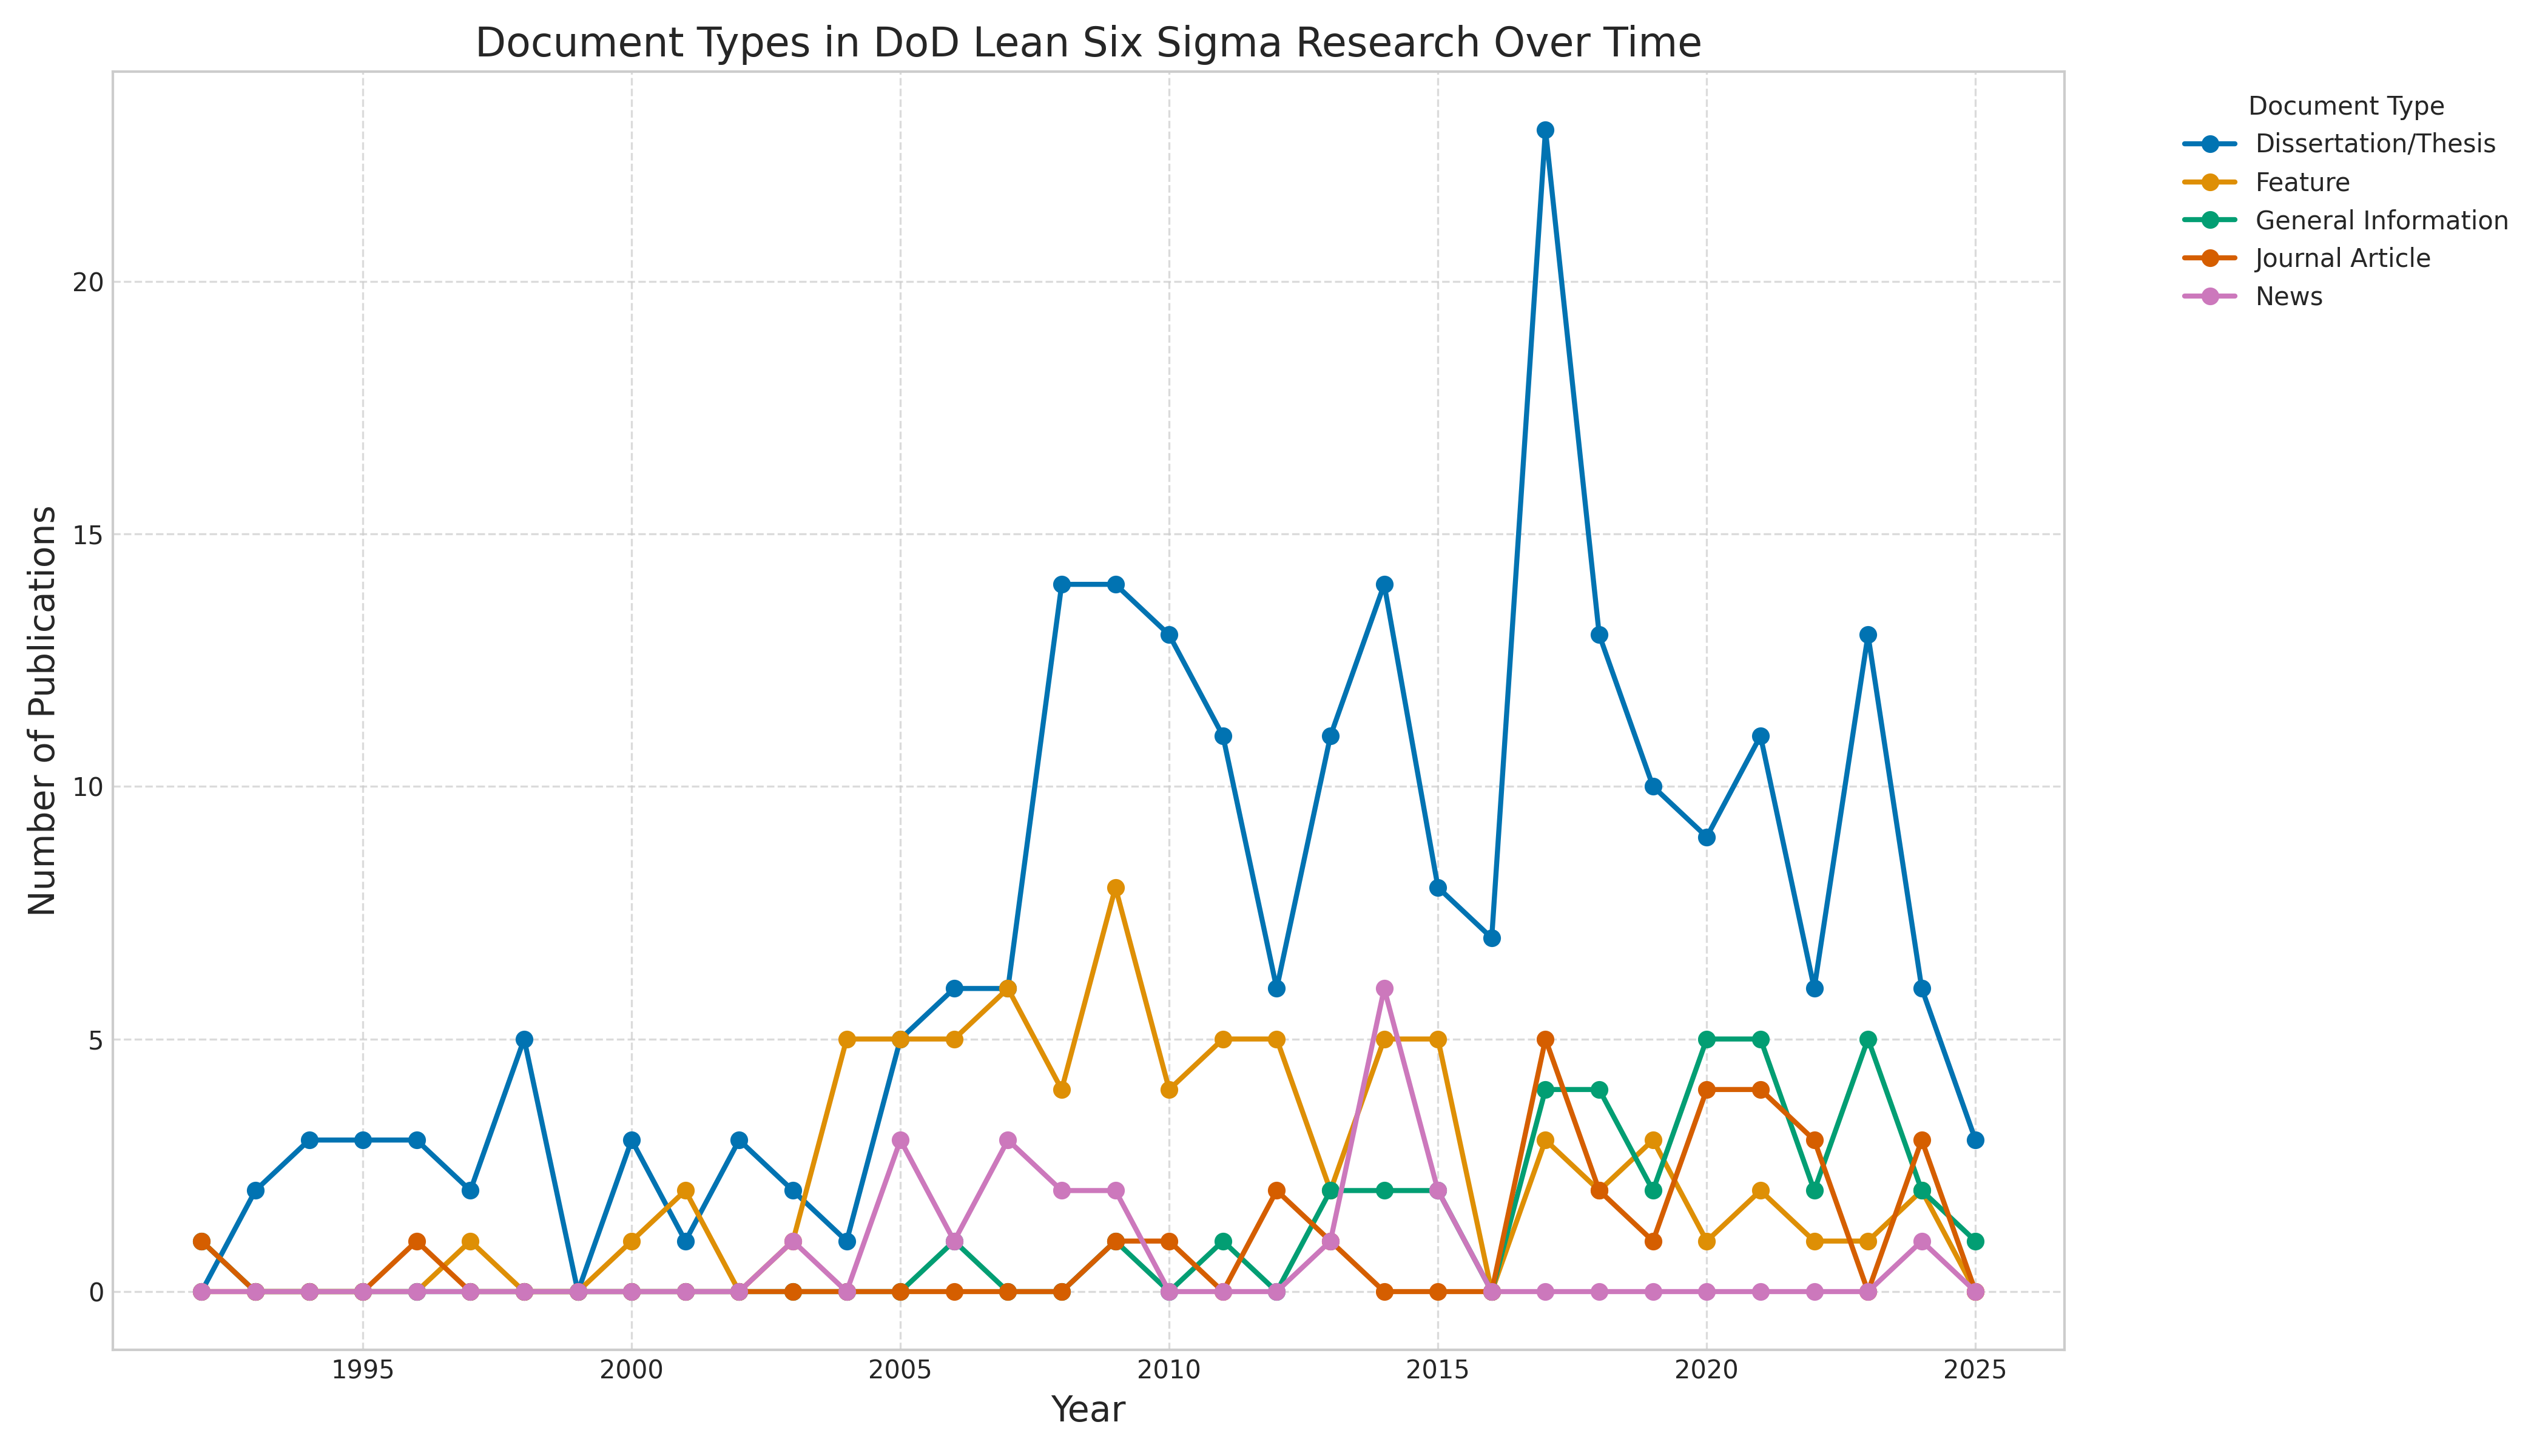
\includegraphics[width=\textwidth,height=0.35\textheight,keepaspectratio]{document_type_trends}
			\caption{Trend over time for the different document types}
			\label{fig:document_type_trend}
		\end{subfigure}
		\caption{Analysis of document types and their trends over time}
		\label{fig:document_analysis}
	\end{figure}


	Analyzing the keywords present in the document abstracts, \figref{fig:keyword_freq} shows that \textit{system}, \textit{process}, and \textit{management} appear with the highest frequency across all documents.

	From the co-occurrence network in \figref{fig:keyword_network}, we observe that \textit{management}, \textit{data}, and \textit{process} have a high betweenness centrality, indicating they serve as important bridges connecting other keywords in the literature. This suggests these concepts play central roles in linking different aspects of lean six sigma implementation within DoD contexts.

	A Latent Dirichlet Allocation method uncovered the following key topic areas, shown in \figref{fig:topics}, \textit{Organization, System, Process/Management,} and \textit{Operation}.

	\begin{figure}[htbp]
		\centering
		\begin{subfigure}[b]{0.32\textwidth}
			\centering
			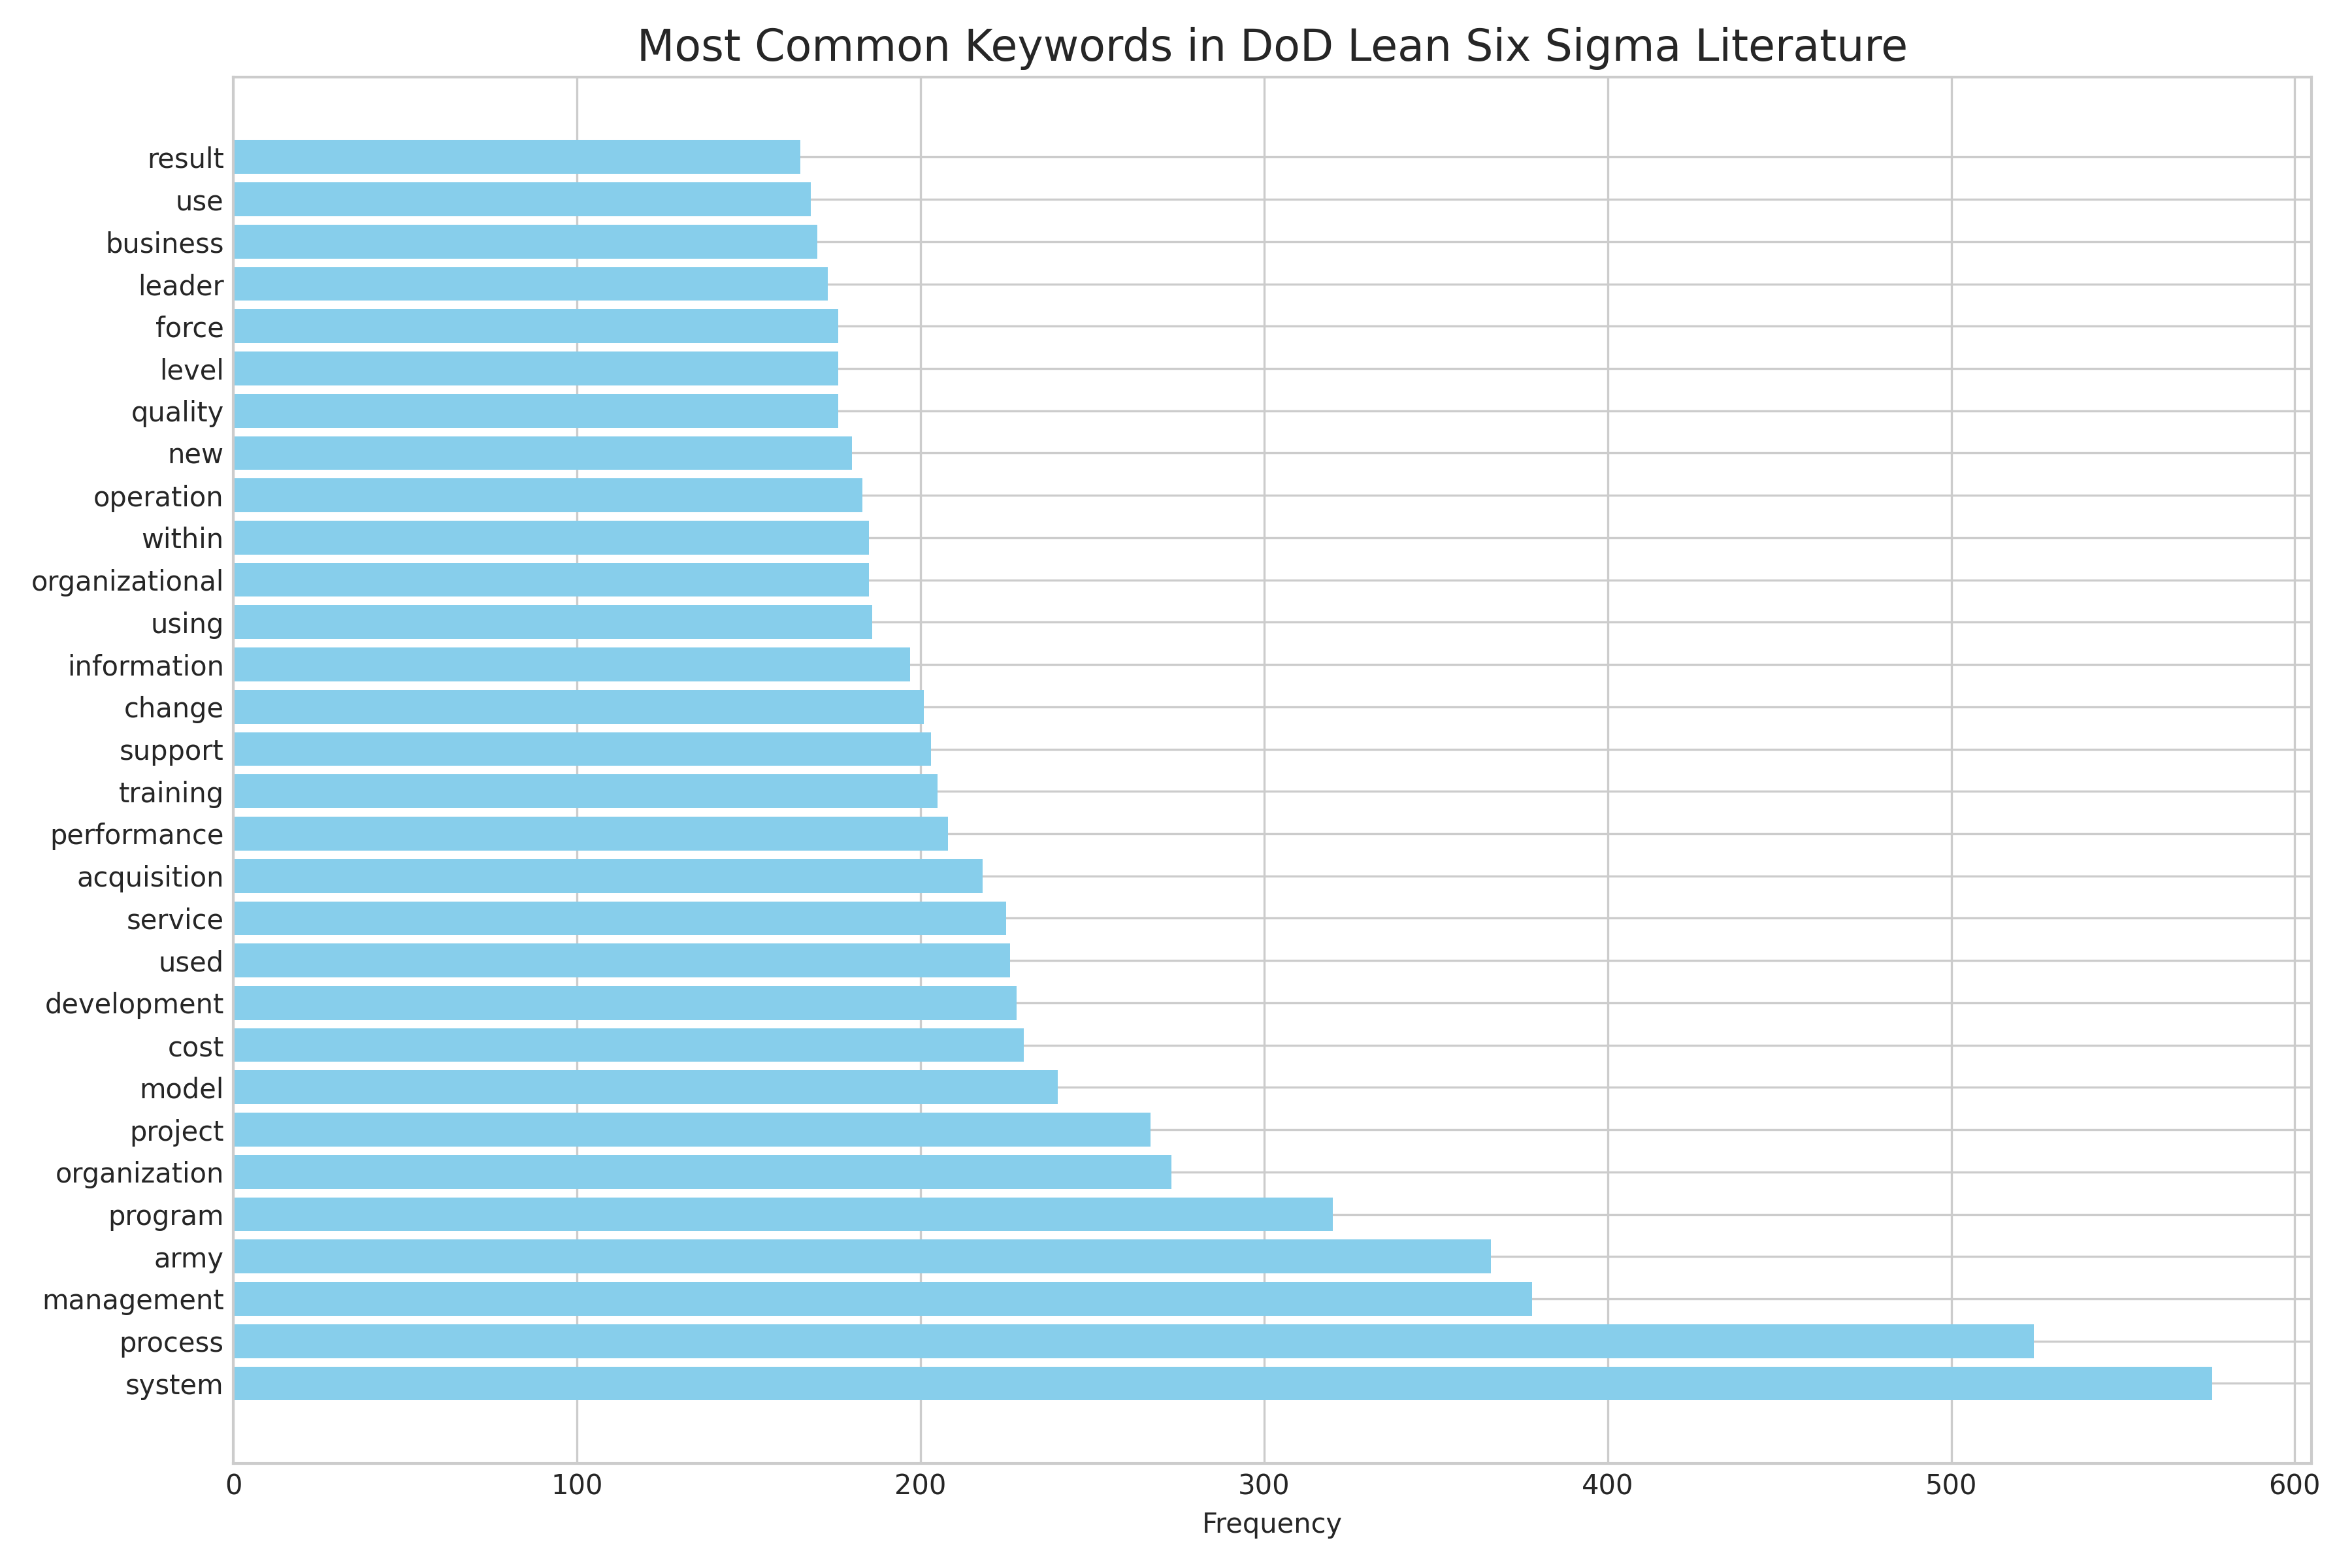
\includegraphics[width=\textwidth,height=0.25\textheight,keepaspectratio]{keyword_frequency}
			\caption{Keyword appearance frequency}
			\label{fig:keyword_freq}
		\end{subfigure}
		\hfill
		\begin{subfigure}[b]{0.32\textwidth}
			\centering
			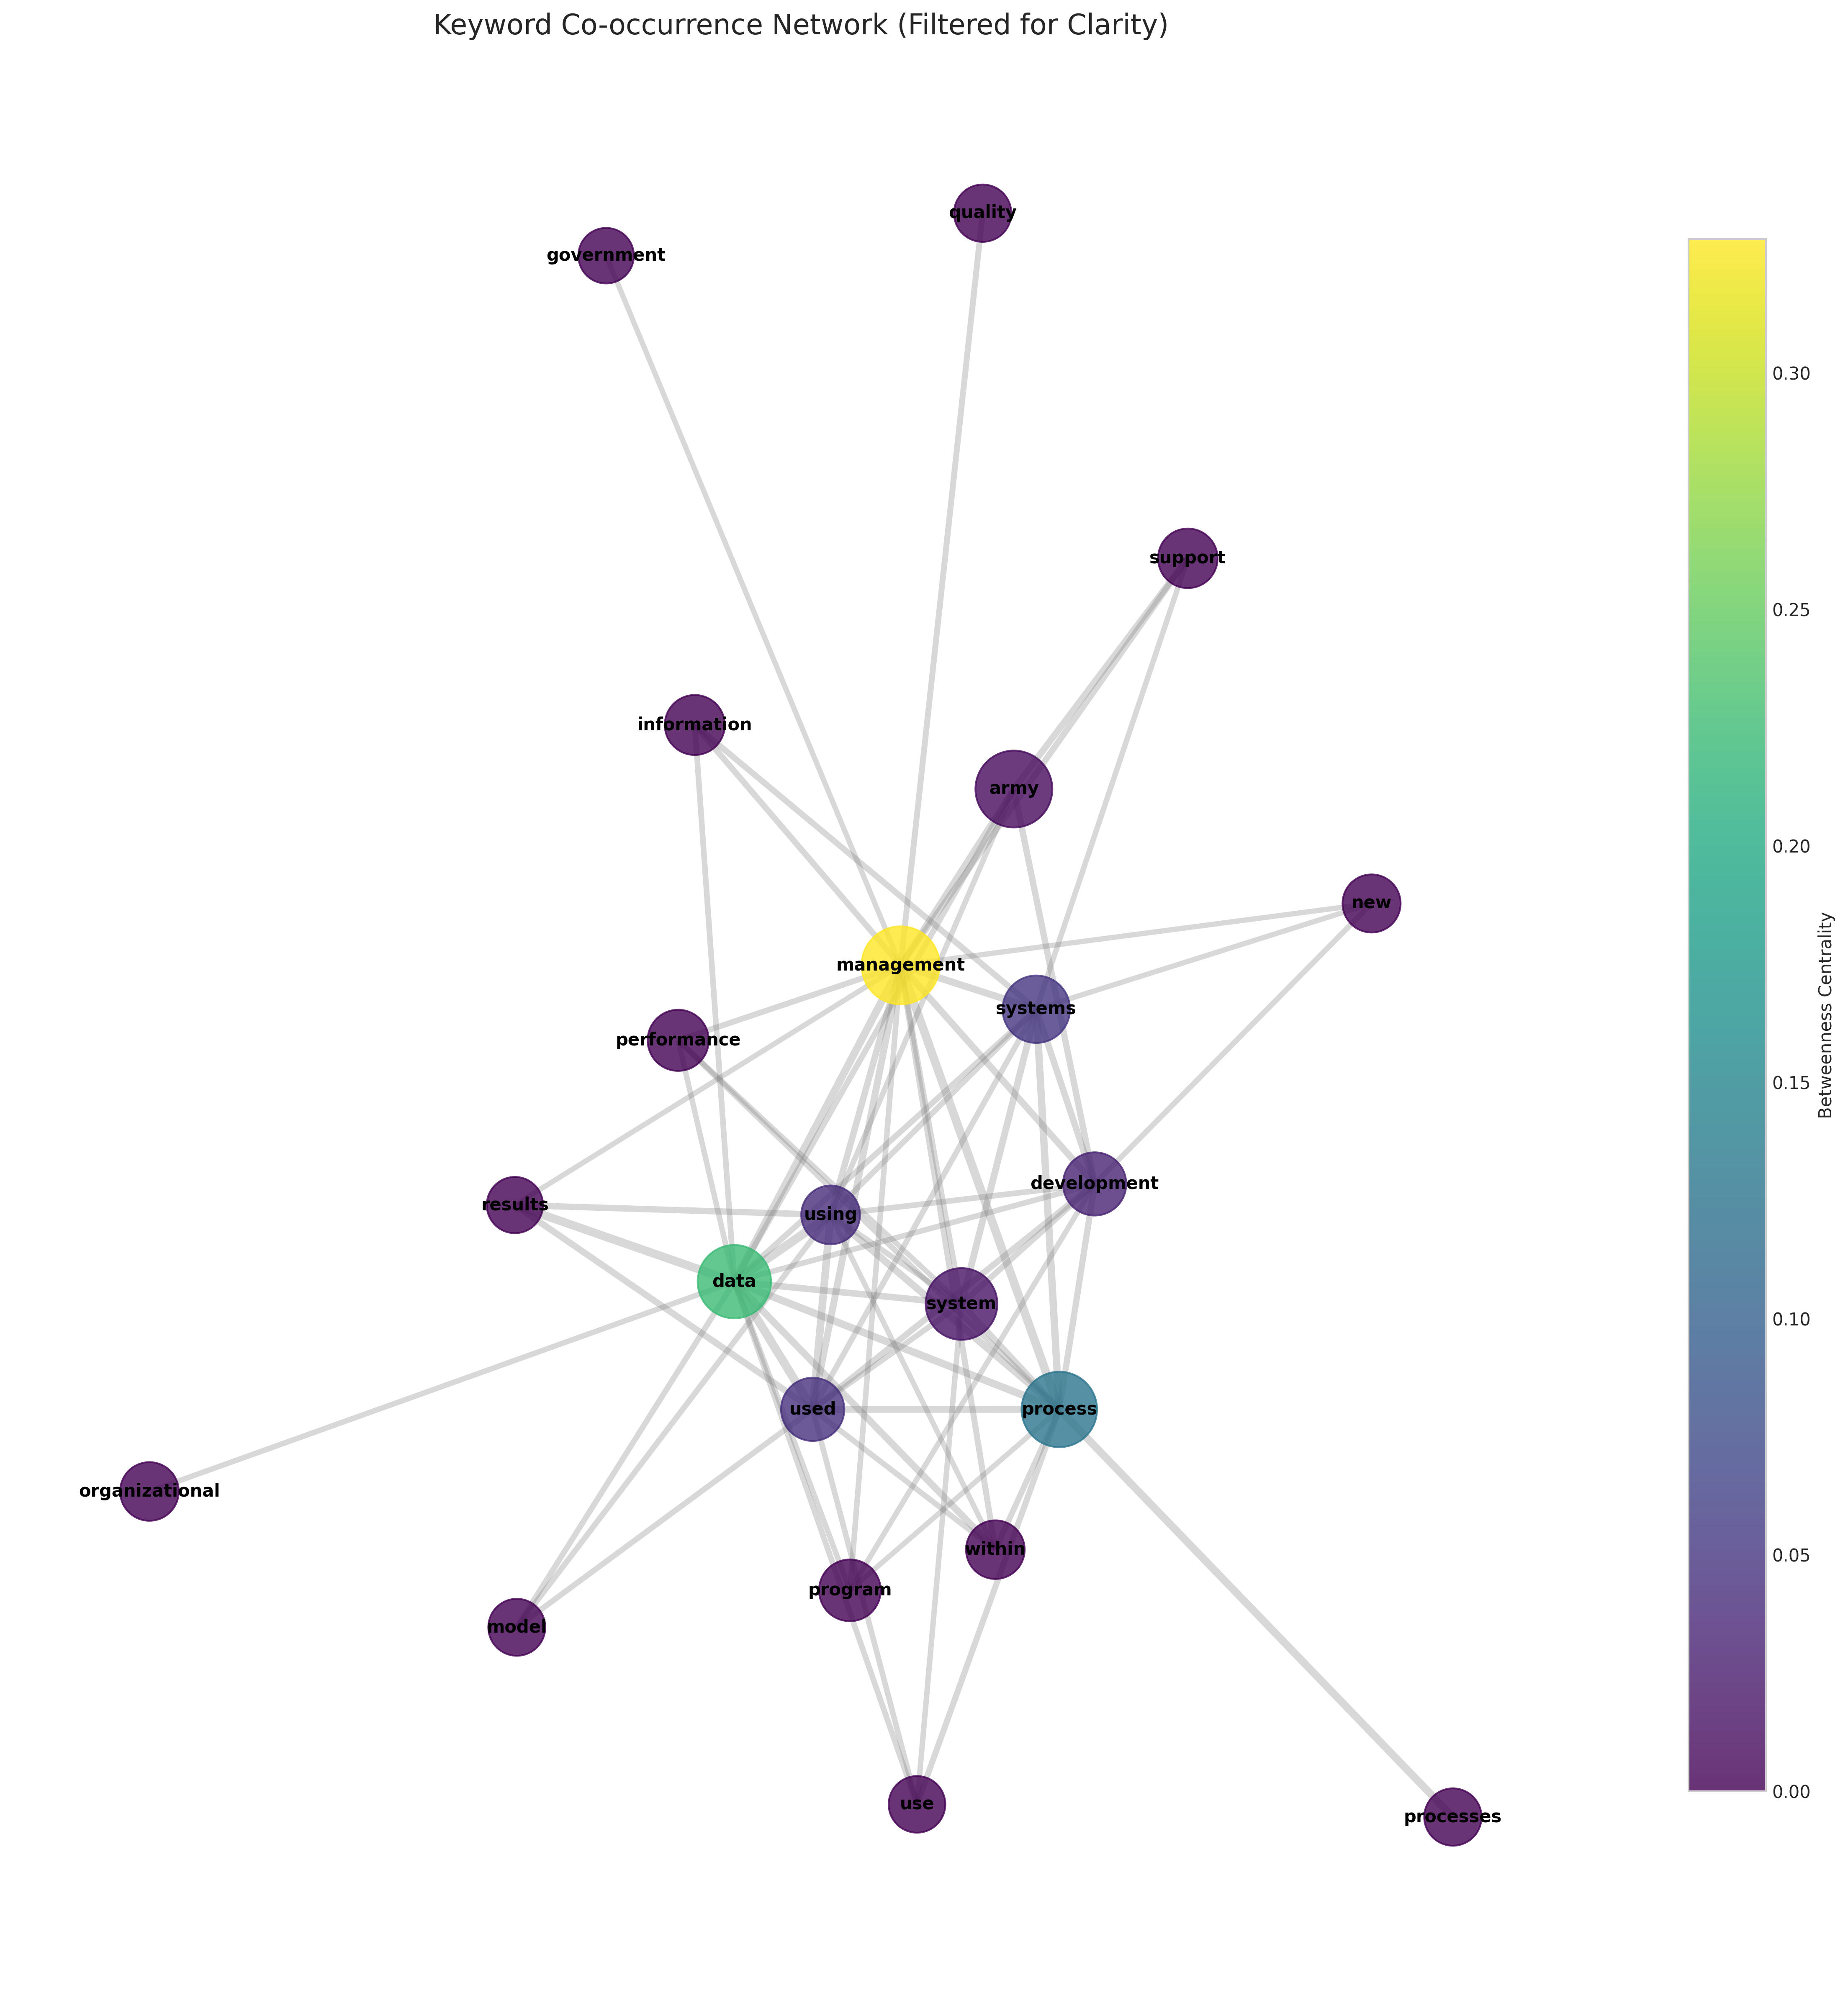
\includegraphics[width=\textwidth,height=0.25\textheight,keepaspectratio]{keyword_network}
			\caption{Keyword co-occurrence network}
			\label{fig:keyword_network}
		\end{subfigure}
		\hfill
		\begin{subfigure}[b]{0.32\textwidth}
			\centering
			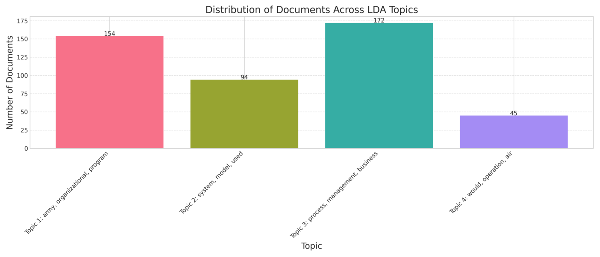
\includegraphics[width=\textwidth,height=0.25\textheight,keepaspectratio]{topic_distribution}
			\caption{Topic distribution from LDA analysis}
			\label{fig:topics}
		\end{subfigure}
		\caption{Keyword analysis and topic modeling results}
		\label{fig:keyword_analysis}
	\end{figure}

	Using all the prior analysis points, the author determined three main themes in the lean six sigma literature: \textit{Management and Leadership, Process Improvement,} and \textit{Continuous Learning}. 
	Using these three themes, a keyword-based categorization algorithm was applied to classify each document according to the most similar theme.

	As visualized in \figref{fig:theme_distribution_bar}, the majority of the papers (54\%) corresponded to the \textit{Management and Leadership} theme, 35.9\% fell into the \textit{Process Improvement} theme, and 9.2\% fell into the \textit{Continuous Learning} theme.
	The distribution of themes over the years is shown in \figref{fig:theme_trends}.

	\begin{figure}[htbp]
		\centering
		\begin{subfigure}[b]{0.48\textwidth}
			\centering
			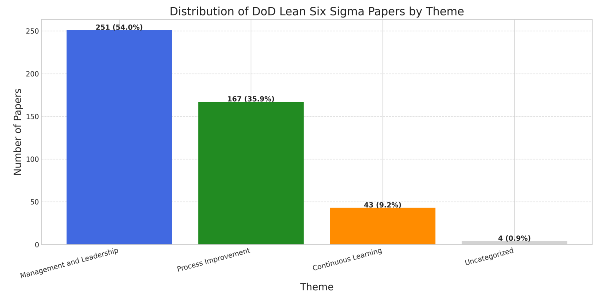
\includegraphics[width=\textwidth,height=0.35\textheight,keepaspectratio]{theme_distribution_bar.pdf}
			\caption{Distribution of themes in the literature}
			\label{fig:theme_distribution_bar}
		\end{subfigure}
		\hfill
		\begin{subfigure}[b]{0.48\textwidth}
			\centering
			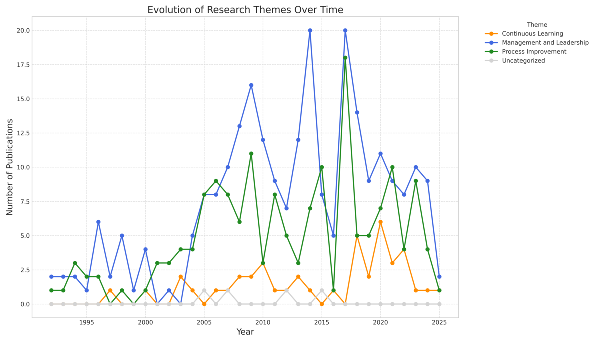
\includegraphics[width=\textwidth,height=0.35\textheight,keepaspectratio]{theme_trends_over_time.pdf}
			\caption{Theme trends over time}
			\label{fig:theme_trends}
		\end{subfigure}
		\caption{Thematic analysis of lean six sigma literature in DoD contexts}
		\label{fig:theme_analysis}
	\end{figure}

	\begin{comment}
		Format:
		- Lean background, how toyota does things

		For each case study:
			- Case study summary
			- Lean analysis

	\end{comment}

	\section{Management and Leadership}

		Toyota's approach to management can be described as Hourensou style management that is multidimensional in nature.
		Managers communicate openly and information travels up, down, and sideways allowing for the necessary flow of information to the correct parties. 

		This is in contrast to traditional North American style of command and control style management where managers delegate out work and information with little input from subordinates.

		In fact, command-and-control style management also makes it difficult to achieve the necessary communication flows to suppliers and external partners.

		Since the DoD follows is composed of various military entities which traditionally operate on this command-and-control style organization, it can be difficult for lean methodologies to take root in such an entrenched system.

		In the following case studies gathered from our literature review, we see examples which offer insight and examples from lean thinking to existing systems in the DoD.


	\subsection{Leadership Development Strategies for Sustaining Organization Performance Through the Upper Echelon Theory \cite{McCants2024}}	

		In \cite{McCants2024}, an analysis is conducted in the Department of Army as to the best practices for transitioning leadership into roles with frequent turnover. 
		Through direct interviews with supervisors of those which transition into the leader roles, the author found that the following skills were prominent for successful managerial transitions:
		\begin{itemize}
			\item Knowledge of an organization during change.
			\item Effective communication skills.
			\item Flexible and adaptive leadership.
			\item Having performance measures.
			\item Formal and informal leader development.
		\end{itemize}

		These themes, although not directly tied to lean thinking in this paper, represent key ideas from the Toyota management style.




	\subsection{Project Engineers on the Frontline: The Impact of Work-Related Stressors and Turnover Intentions: A Correlational Study \cite{Turner2024}}

		In \cite{Turner2024}, the author conducts surveys on project engineers who have worked in the DoD or a company which contracted for the DoD in order to analyze the effect of work related stressors and employee turnover.
		Project engineers in this work were engineers directly managing planning, budgets, execution and delivery of DoD projects.
		
		The author found a strong positive correlation between work related stress and turnover intention among the surveyed individuals.
		In addition, the author found job tension had a significant impact on turnover considerations by the engineers.

		By going to the source, the author was able to identify one of the root causes of a serious problem in DoD projects. 
		The author suggested the changes of leadership development, supportive culture, and proper resources could improve the current state. 

		These findings align with lean thinking, as Toyota managers will attempt to create a leveled work flow to avoid the deadly waste of overburden on it's employees. 
	


	\subsection{Understanding the Contracting Environment in the AFSB: Army Logistician \cite{Carlstedt2020}}

		The article of \cite{Carlstedt2020} provides insight into how the Army, a DoD organization, manages relations and contracts with it's suppliers.
		The Army contracts out critical work such as dining halls, bus drivers, and tailoring, all of which contracts careful planning and rule setting between the Army Field Support Brigade (AFSB) and the contract supplier. 

		A Requiring Activity (RA) identifies shortfalls requiring contracted solutions and develops the Performance Work Statement (PWS). 
		The Contracting Officer's Representative (COR) serves as liaison between the Contracting Officer (KO) and contractor (KTR), while Quality Assurance Evaluators (QAEs) monitor performance according to the Quality Assurance Surveillance Plan (QASP). 

		Contract accountability is maintained through regular Performance Management Reviews (PMRs) and Contract Management Reviews (CMRs), with commanders having multiple tools to address substandard performance including Noncompliance Reporting, invoice deductions, negative CPARS assessments, and contract re-competition. 
		Importantly, the article emphasizes that commanders must balance strict enforcement with maintaining a healthy Defense Industrial Base, recognizing contractors as valuable strategic partners.

		The emphasis on standardized documents and knowledge of those documents for contract managers demonstrate important strategies for a lean organization.
		The regular reviews (PMRs and CMRs) also create the feedback loops necessary for continuous improvement.

		The balanced approach to contractor relationships reflects Toyota's keiretsu philosophy of building long-term partnerships with suppliers rather than purely transactional relationships. 
		By emphasizing both accountability and partnership, the AFSB approach aligns with Toyota's respect for partners in the value stream. 


	\section{Process Improvement}

		Process improvement is a fundamental task for any lean organization. 
		Improvement comes from building a culture of kaisen (continuous improvement), where non-value adding steps (waste) in a process can be identified and removed. In the following literature we examine a few ways opportunities for process improvement have been implemented in the DoD.

		\section{The Army's Process to Evaluate Costs Versus Benefits: A Case Study on the Change of Command Ceremonies \cite{Malin2020}}

			The Army holds many traditional ceremonies and events meant to commemorate special occasions. 
			One such ceremony is the change of command (COC) ceremony which is held at various levels within an Army unit to welcome new leadership. 
			Since a command position is a two year assignment and each of the four sub-organizations in an Army division (division, brigade, battalion, company) must execute a COC this leads to an excess of wasted time for army personnel.

			The author of \cite{Malin2020} found through interviews with key leadership involved with the celebrations organization that the Department of the Army lack a proper process to evaluate the loss costs for COC ceremonies.
			These losses stem from mandatory attendance of military personnel, firing of weaponry, and planning resources.

			Production loss costs represent the cost that the organization incurs when an employee's duty or productivity is suspended by a disruption. In the case of change of command ceremonies, these costs can range from \$17,964.44 per hour for a company-sized unit to \$404,200 per hour for a division-sized unit. 
			Despite the significant resources involved, Malin's research discovered that the Army did not provide the necessary support for senior advisors to evaluate the value of change of command ceremonies against these costs.

			The study concluded with recommendations for a training-based solution and tools as in \figref{fig:loss_tool}, that would help leaders better understand and implement cost-benefit analyses for these ceremonies. 
			
			\begin{figure}[htbp]
			\centering
			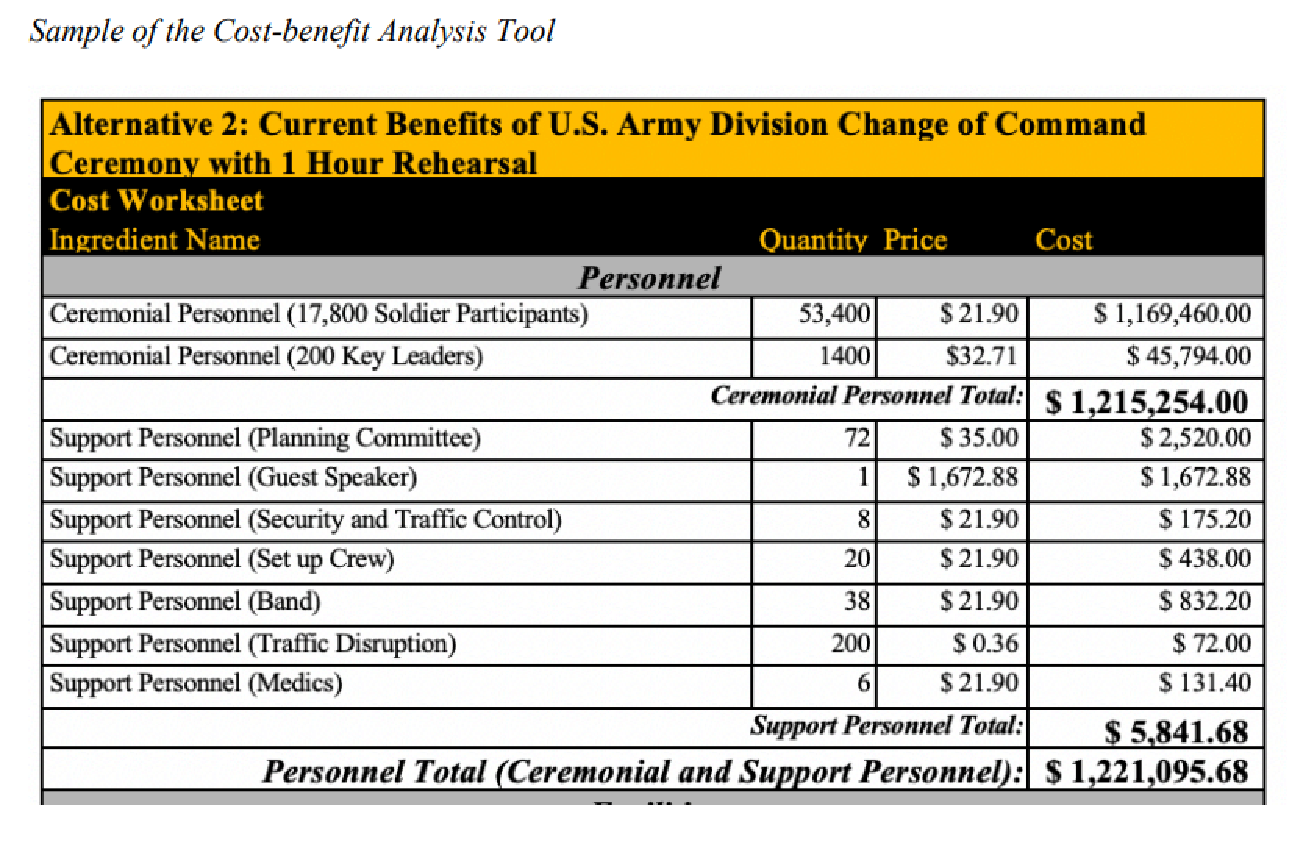
\includegraphics[width=0.4\linewidth,height=0.4\textheight,keepaspectratio]{figures/cost_tool.pdf}
			\caption{Proposed cost tool of \cite{Malin2020}, demonstrating how Army can value Production Loss Costs for different situations.}
			\label{fig:loss_tool}
			\end{figure}

		

		\section{Improving Depot Repair Lead Time Using Lean Six Sigma \cite{Richmond2023}}

			In \cite{Richmond2023}, the author applies Lean Six Sigma methodology to address excessive lead times in aircraft component repairs at a Naval Fleet Readiness Center Southeast (FRCSE) depot. 

			The author makes use of the DMAIC (Define, Measure, Analyze, Improve, Control) framework in order to identify bottlenecks in the repair process. 
			The research revealed that the mean repair turnaround time was 132 days—substantially longer than the expected 55-day timeline. 
			By collecting time data for each process step and utilizing value stream mapping, the author discovered that non-value-added activities comprised approximately 85\% of the total repair time. The primary contributors to delays included: excessive inventory queues between work centers, disorganized work areas, inefficient routing of components, and a lack of standardized work procedures.

			

			The results of these interventions were substantial, with repair lead time reduced by 44\% and a corresponding 33\% increase in repair throughput capacity. The annualized cost avoidance was calculated at \$1.9 million.

			This case study exemplifies core Toyota Production System principles in action, particularly the elimination of muda (waste) in all its forms. The author's approach aligns with lean thinking by identifying and addressing transportation, inventory, motion, waiting, overprocessing, overproduction, and defects within the repair process. 

			The emphasis on reducing non-value-added time rather than pushing for faster processing of value-added activities reflects the true essence of lean thinking—identifying and eliminating waste rather than simply pushing workers to perform faster. The case demonstrates how a structured Lean Six Sigma approach can transform a cumbersome, inefficient process into one that delivers greater value with fewer resources, even within the constraints of a government maintenance facility.




		\section{Analyzing Factors That Contribute to Cost Overruns on Department of Defense (DoD) Contractor Programs \cite{FunchesAllen2025}}






	\section{Continuous Learning}

		Building a culture of continuous learning through hansai and kaisen is a cornerstone of the Toyota Way.
		In the digital age, this learning culture can be amplified through digitization of organizational knowledge and data.

		However, a poor approach to such systems can result in the development of waste if information is not easily accessible at the right time, by the right people.

		In the following case studies we see how DoD groups are addressing the existing methods of knowledge base management and data collection to create a lean and effective organization.

		\section{Engineering Management Tool for Minimizing Errors and Costs in Diagnosing PTSD in Veterans \cite{Le2023}}


		\section{Knowledge Management Implementation in U.S. Army Headquarters: A Case Study \cite{VanLaar2023}}


		\section{Stitching the Army's Data Fabric \cite{Patel2021}}






\newpage

\bibliographystyle{IEEEtran}
\nocite{*}
\bibliography{/project/src/ref}

\end{document}